\newpage
\section{Running XDD Programs}\label{running-xdd-programs}

XDD programs include XDD itself, the timeserver program, and the gettime program. Example command lines are given in Appendix B and are also contained in a file called tests.txt in the distribution bin directory.

\subsection{XDD Command Line Arguments Synopsis}\label{xdd-command-line-arguments-synopsis}

\begin{quote}
xdd

-blocksize \emph{{[}target \textless target\#\textgreater{]} number\_of\_bytes\_per\_block}

-bytes \emph{{[}target \textless target\#\textgreater{]} number\_of\_bytes\_to\_xfer\_per\_pass}

\emph{-}combinedout \emph{filename}

-createnewfiles \emph{{[}target \#{]}}

\emph{-}csvout \emph{filename}

-datapattern \emph{{[}target \textless target\#\textgreater{]}}

\emph{character\_pattern --or-}

\emph{``}\textbf{random}\emph{'' --or-}

\emph{``}\textbf{sequenced}\emph{'' --or-}

\emph{``}\textbf{prefix}\emph{'' --or-}

\emph{``}\textbf{inverse}\emph{'' --or-}

\emph{``}\textbf{ascii} \textless{}\emph{string}\textgreater'' \emph{--or-}

\emph{``}\textbf{hex} \textless{}\emph{hex digits 0-9, a-f or A-F}\textgreater{}\emph{'' --or-}

\emph{``}\textbf{replicate}\emph{'' --or-}

\emph{``}\textbf{lfpat}\emph{'' --or-}

\emph{``}\textbf{ltpat}\emph{'' --or-}

\emph{``}\textbf{cjtpat}\emph{'' --or-}

\emph{``}\textbf{crpat}\emph{'' --or-}

\emph{``}\textbf{cspat}\emph{''}

-deletefile \emph{{[}target \textless target\#\textgreater{]}}

-deskew

-dio \emph{{[}target \textless target\#\textgreater{]}}

-dryrun

-endtoend \emph{{[}target \textless target\#\textgreater{]}}

\textbf{issource \textbar{} isdestination}

\textbf{port} \emph{\#}

\textbf{portcount} \emph{\#}

\textbf{destination} \emph{hostname:base\_port,number\_of\_ports}

-errout \emph{filename}

-flushwrite \emph{\#ops}

-fullhelp

-heartbeat \emph{{[}target \textless target\#\textgreater{]} \#seconds\textbar hostname\textbar target\textbar tod\textbar elapsed\textbar lf\textbar{}}

\emph{output \textless filename\textgreater\textbar bw\textbar ops\textbar bytes\textbar kbytes\textbar mbytes\textbar gbytes\textbar iops\textbar pct\textbar etc}

-help \emph{option\_name}

-id \textbf{commandline} - or - \emph{``id\_string''}

-kbytes \emph{{[}target \textless target\#\textgreater{]} number\_of\_kilobytes\_to\_transfer}

\emph{-}lockstep \emph{\textless master\_target\textgreater{} \textless slave\_target\textgreater{}}

\emph{\textless when\textgreater{} \textless howlong\textgreater{}}

\emph{\textless what\textgreater{} \textless howmuch\textgreater{}}

\emph{\textless startup\textgreater{} \textless completion\textgreater{}}

-looseordering \emph{{[}target \textless target\#\textgreater{]}}

-maxall

-maxerrors \emph{number\_of\_errors}

-maxerrorstoprint \emph{number\_of\_errors\_to\_print}

-maxpri

-mbytes \emph{{[}target \textless target\#\textgreater{]} number\_of\_megabytes\_to\_transfer}

-memalign \emph{{[}target \textless target\#\textgreater{]} alignment\_value\_in\_bytes}

-minall

-nomemlock

-noordering \emph{{[}target \textless target\#\textgreater{]}}

-noproclock

-numreqs \emph{{[}target \textless target\#\textgreater{]} number\_of\_requests\_to\_perform}

-op \emph{{[}target \textless target\#\textgreater{]} rea}d\textbar{}\emph{write\textbar noop}

-ordering \emph{{[}target \textless target\#\textgreater{]} \textless storage\textbar network\textbar both\textgreater{} \textless serial\textbar loose\textbar none\textgreater{}}

-output \emph{filename}

-outputformat \textbf{add} \emph{\textbar{}} \textbf{new} \emph{\textless format\_id\_string\textgreater{}}

-passdelay \#.\#\emph{seconds}

-passes \emph{number\_of\_passes}

-passoffset \emph{{[}target \textless target\#\textgreater{]} offset\_in\_blocks}

-preallocate \emph{{[}target \textless target\#\textgreater{]} number\_of\_bytes}

-processlock

-processor \emph{{[}target \textless target\#\textgreater{]} processor\_number}

-queuedepth \emph{{[}target \textless target\#\textgreater{]} number\_of\_commands\_per\_target}

-qthreadinfo

-randomize \emph{{[}target \textless target\#\textgreater{]}}

-recreatefiles \emph{{[}target \#{]}}

-reopen \emph{{[}target \#{]}}

-reportthreshold \emph{{[}target \#{]} \textless\#.\#\textgreater{}}

-restart \emph{{[}target \textless target\#\textgreater{]}}

\textbf{enable}

\textbf{frequency} \emph{\textless seconds\textgreater{}}

\textbf{file} \emph{\textless name\_of\_restart\_file\textgreater{}}

\textbf{offset} \emph{\textless offset\_in\_bytes\textgreater{}}

-roundrobin \# \emph{\textbar{} `all'}

-runtime \#.\#\emph{seconds}

-rwratio \emph{{[}target \#{]} \textless readwriteratio\textgreater{}}

-seek \emph{{[}target \textless target\#\textgreater{]}}

\textbf{save} \emph{filename}

\textbf{load} \emph{filename}

\textbf{disthist} \emph{\#}

\textbf{seekhist} \emph{\#}

\textbf{random}

\textbf{range \#}

\textbf{stagger}

\textbf{interleave \#}

\textbf{seed \#}

\textbf{none}

-serialordering \emph{{[}target \textless target\#\textgreater{]}}

-setup \emph{setup\_filename}

-sgio

-sharedmemory \emph{{[}target \textless target\#\textgreater{]}}

-singleproc \emph{processor\_number}

-startdelay \emph{{[}target \textless target\#\textgreater{]} \#.\#seconds}

-startoffset \emph{{[}target \textless target\#\textgreater{]} starting\_block\_number}

-starttime \emph{\#seconds}

-starttrigger \emph{targetA target\textgreater{} \textbf{time\textbar op\textbar percent\textbar mbytes\textbar kbytes} \#}

-stoponerror

-stoptrigger \emph{targetA target\textgreater{} \textbf{time\textbar op\textbar percent\textbar mbytes\textbar kbytes} \#}

-syncio \emph{number}

-syncwrite \emph{{[}target \textless target\#\textgreater{]} number}

-target \emph{filename}

-targetdir \emph{{[}target \textless target\#\textgreater{]} directoryname}

-targetoffset \emph{{[}target \textless target\#\textgreater{]} offset\_in\_blocks}

-targets \emph{N name1 name2 \ldots{} nameN}

-targetstartdelay \emph{{[}target \textless target\#\textgreater{]} \#.\#seconds}

-throttle \emph{{[}target \textless target\#\textgreater{]}}

\textbf{ops} \emph{operations/sec}

\textbf{bw} \emph{megabytes/second}

-timelimit \emph{{[}target \textless target\#\textgreater{]} \#.\#seconds\_per\_pass}

-timeserver

\textbf{host} \emph{hostname}

\textbf{port} \emph{port\#}

\textbf{bounce} \emph{bounce\_count}

-timestamps \emph{{[}target \textless target\#\textgreater{]}}

\textbf{output} \emph{output\_filename\_prefix}

\textbf{summary}

\textbf{detailed}

\textbf{normalize}

\textbf{summary}

\textbf{wrap}

\textbf{oneshot}

\textbf{size \#}

\textbf{triggertime} \emph{\#seconds}

\textbf{triggerop} \emph{operation\#}

\textbf{append}

\textbf{dump} \emph{dump\_filename\_prefix}

-verbose

-verify \emph{{[}target \textless target\#\textgreater{]}}

\textbf{location}

\textbf{contents}

-version
\end{quote}

\subsection{Detailed Option Specifications}\label{detailed-option-specifications}

\textbf{-blocksize} specifies the number of bytes per block. This defaults to 1024 bytes per block. Block sizes must be powers of 2 or the results are unpredictable.

\textbf{-bytes} specifies the number of bytes to transfer per pass. This can be any positive number up to 2\textsuperscript{64}-1. See also: -\textbf{kbytes} and \textbf{-mbytes}.

\textbf{-combinedout} \emph{filename} will append just the ``Combined'' results output to the file specified by \emph{filename}. This allows for collecting the Combined performance data from multiple runs in a single file. This does not include error messages. See the \textbf{--errout} option for more information on redirecting error output.

Scope: Global

-\textbf{createnewfiles} will cause new target files to be created for each pass in an XDD run. Each new file has the file name that was given as the target file name but it is appended with a number that represents the pass in which it was created. It is not a good idea to run this on a target ``device'' file because the new target will get recreated as regular files and not a special device files.

\textbf{-csvout} \emph{filename} will send all the results output to the file specified by \emph{filename} similar to the --output option. The difference between -csv output and the normal output is that this is a Comma Separated Values file that is directly importable into MS Excel. This does not include error messages. See the \textbf{--errout} option for more information on redirecting error output.

Scope: Global

\textbf{-datapattern} specifies either a single byte data pattern character or a special operator as described below. (\emph{Note: This option was formerly called --pattern})

\begin{itemize}
\item
  If the operator ``\textbf{random}'' is specified then a random data pattern is generated in the entire I/O buffer.
\item
  If the operator ``\textbf{sequenced}'' is specified, then the data pattern will be sequential 64-bit integers starting with the current block address times the size of a 64-bit integer. It should be noted that writing this sequenced pattern to the device will result in additional CPU overhead that may affect overall performance. Similarly, for read operations, if the ``\textbf{sequenced}'' data pattern is specified, the data is checked to see if the data read is in fact what was expected.
\item
  If the word ``\textbf{prefix}'' is specified for the pattern then the specified hex digits will be placed in the upper N bits of the 64-bit pattern
\item
  If the operator ``\textbf{inverse}'' is specified for the pattern then the actual pattern will be the 1\textquotesingle s compliment of the specified pattern
\item
  If the word ``\textbf{ascii}'' is used as the data pattern, then the data pattern will be the string specified after the ``\textbf{ascii}'' operator. The string is only written once at the beginning of the I/O buffer and is not repeatedly copied throughout the I/O buffer.
\item
  If the word \textbf{``hex''} is specified then the following hex characters \textless0-9,a-f or A-F\textgreater{} are used as the pattern
\item
  If the word ``\textbf{replicate}'' is specified then whatever pattern was specified is replicated throughout the buffer
\item
  If the word ``\textbf{lfpat}'' is specified then the low-frequency 8B/10B pattern is used
\item
  If the word ``\textbf{ltpat}'' is specified then the low-transition 8B/10B pattern is used
\item
  If the word ``\textbf{cjtpat}'' is specified then the compliant jitter 8B/10B pattern is used
\item
  If the word ``\textbf{crpat}'' is specified then the compliant random 8B/10B pattern is used
\item
  If the word ``\textbf{cspat}'' is specified then the compliant sequential 8B/10B pattern is used
\item
  The default data pattern is all binary 0\textquotesingle s
\end{itemize}

\textbf{-deletefile} will cause the target file to be deleted at the end of a run. To have files deleted and recreated between passes, see the \textbf{--recreatefiles} option.

\textbf{-deskew} will adjust the performance calculations to deskew the results. See section on Deskew for more information.

Scope: Global

\textbf{-dio} will turn on the DIRECT IO option when accessing a regular file. This option cannot be used when accessing special device files. Certain blocksize, and alignment restrictions apply and will cause problems if the wrong combination of block size and offsets are chosen.

\textbf{-endtoend} specifies that the target device will participate in an End-to-End operation. There are two sides to an End-to-End (aka e2e) operation: the \emph{source} and the \emph{destination}. It takes two concurrent instances of \emph{XDD} to perform an e2e operation: one running on the \emph{source} side and one running on the \emph{destination} side. The instance of \emph{XDD} on the \emph{source} side of the e2e operation will read the specified target file/device and transfer the data over a TCP/IP socket to the instance of \emph{XDD} on the \emph{destination} side. The \emph{destination} instance of \emph{XDD} will receive the incoming data and write it to its specified target file/device. See section on Examples for more information.

The e2e option has the following operators:

\begin{itemize}
\item
  If the operator ``\textbf{issource}'' is specified then this particular instance of \emph{XDD} assumes that it is on the \emph{source} side of an e2e operation.
\item
  If the operator ``\textbf{isdestination}'' is specified then this particular instance of \emph{XDD} assumes that it is on the \emph{destination} side of an e2e operation.
\item
  The operator ``\textbf{destination} \emph{hostname{[}:baseport{[},\#ports{]}{]}}'' specifies the name of the host on the \emph{destination} side of an e2e operation. The \emph{hostname} can be specified as a name or an IP Address. Optionally, the baseport to use and the number of ports to use starting from the base port number can also be specified as indicated. It is necessary to specify this address on both instances of \emph{XDD}, \emph{source} side \ul{and} \emph{destination} side, in order to explicitly define the correct network interface to use for the data transfer. Furthermore, if the baseport and number of ports is specified, the queue depth will be implied thereby eliminating the need to specify the ``-queuedepth'' option.
\item
  The ``\textbf{port} \#'' defines the specific port to use for the data transfer. In the event that multiple threads are used on each side of the e2e operation (i.e. --queuedepth 48) then the port number becomes the base port number and is incremented by 1 for each subsequent QThread. For example, if ``--queuedepth 4'' is specified along with ``--e2e port 3010'' then the port assignments will consume port numbers 3010, 3011, 3012, and 3013 for QThreads 0, 1, 2, and 3 respectively. For this type of operation it is important to choose a base port number that has free ports within the range of ports that will be consumed.
\end{itemize}

\textbf{-errout} \emph{filename} will send all the error message output to the file specified by \emph{filename}. This does not include normal results output. See the \textbf{--output} option for more information on redirecting results output.

Scope: Global

\textbf{-flushwrite} will force a sync() operation to occur every so many write operations as specified by the associated argument to this option.

\textbf{-fullhelp} will display a list of these options \emph{and} a one line explanation of each.

Scope: Global

\textbf{-heartbeat} \emph{{[}target \textless target\#\textgreater{]}} \textbf{\textless{}}\emph{suboption}\textbf{\textgreater{}}

Where ``\emph{suboption}'' can be one of the following:

\begin{itemize}
\item
  \emph{\#seconds} will display Pass Number and requested information for each target I/O thread every N seconds where N is specified as \emph{\#seconds}.
\item
  \emph{hostname -} Will include the name of the host machine that the instance of XDD is running on. The ``hostname'' appears at the beginning of the output line and is prefixed by ``HOST''.
\item
  \emph{target -} Will include the target number before each output grouping. The target number is followed by ``tgt'' to indicate that it is the Target number.
\item
  \emph{tod} - Will include the current Time of Day on each heartbeat update. The Time of Day appears at the beginning of the output line and is prefixed by ``TOD''.
\item
  \emph{elapsed} - Will include the elapsed number of seconds for the run on each heartbeat update. The Elapsed Seconds appears at the beginning of the output line and is prefixed by ``ELAPSED''.
\item
  \emph{lf} - Will include a ``line feed'' character at the end of each heartbeat output line.
\item
  \emph{output \textless filename\_prefix\textgreater{}} - will send all heartbeat updates to a file with a name of the form ``\emph{filename\_prefix}.T\#\#\#\#.csv'' where ``\emph{filename\_prefix}'' is the argument to the \textbf{--hb output} option and T\#\#\#\# is the letter ``T'' followed by a four-digit Target Number. The heartbeat output is presented as an ASCII string of comma-separated values hence the filename will end with a file extension of ``.csv'' so that it can be more easily imported into a spreadsheet. Only the heartbeat values for the specific Target is written to the heartbeat output file.
\item
  \emph{bw} - Will display the aggregate bandwidth of each target thread on each heartbeat update. The bandwidth is expressed in units of 10\textsuperscript{6} or Mega Bytes per second.
\item
  \emph{ops} - Will display the total number of completed I/O operations on each heartbeat update.
\item
  \emph{bytes} - Will display the current total number of bytes transferred on each heartbeat update.
\item
  \emph{kbytes} - Will display the current total number of Kilo Bytes (10\textsuperscript{3} bytes) transferred on each heartbeat update.
\item
  \emph{mbytes} - Will display the current total number of Mega Bytes (10\textsuperscript{6} bytes) transferred on each heartbeat update.
\item
  \emph{gbytes} - Will display the current total number of Kilo Bytes (10\textsuperscript{9} bytes) transferred on each heartbeat update.
\item
  \emph{iops} - Will display the current aggregate I/O Operations per Second on each heartbeat update.
\item
  \emph{pct} - Will display the current Percent of I/O Operations Completed on each heartbeat update.
\item
  \emph{etc} - Will display the current Estimated Time to Completion on each heartbeat update.
\end{itemize}

Scope: Target Specific

\textbf{-id} allows the user to specify an ASCII string to be displayed in the output in order to identify the run. If the word \textbf{commandline} is used as the character string then the input command line is used as the id. Multiple instances of the -id option will concatenate each specified id to the previous one.

Scope: Global

\textbf{-kbytes} specifies the integer number of kilobytes to transfer on each pass. In this case, one kilobyte is equal to 1024 bytes. If the --\textbf{numreqs} option is also specified, --\textbf{numreqs} takes precedence.

See also: -\textbf{mbytes} and \textbf{-bytes}.

\textbf{-lockstep} \emph{\textless master\_target\textgreater{} \textless slave\_target\textgreater{} \textless when\textgreater{} \textless howlong\textgreater{} \textless what\textgreater{} \textless howmuch\textgreater{} \textless startup\textgreater{} \textless completion\textgreater{}\\
}Where

\emph{"\textbf{master\_target}"} is the target that tells the slave when to do something.\emph{\hfill\break
~~~~~~ "\textbf{slave\_target}"} is the target that responds to requests from the master.\emph{\hfill\break
~~~~~~ "\textbf{when}"} specifies when the master should tell the slave to do something.

\begin{quote}
The word "\emph{\textbf{when}}" should be replaced with the word:\\
\strut ~~~~~~~~~~~ "\textbf{time}"\\
\strut ~~~~~~~~~~~ "\textbf{op}"\\
\strut ~~~~~~~~~~~ "\textbf{percent}"\\
\strut ~~~~~~~~~~~ "\textbf{mbytes}"\\
\strut ~~~~~~~~~~~ "\textbf{kbytes}"

\emph{"\textbf{howlong}"} is either the number of seconds, number of operations, ...etc.
\end{quote}

\begin{itemize}
\item
  The interval time in seconds (a floating point number) between task requests from the master to the slave. i.e. if this number were 2.3 then at every 2.3-second interval the master would request the slave to perform its task.
\item
  The operation number that defines the interval on which the master will request the slave to perform its task. i.e. if the operation number is set to 8 then upon completion of every 8 (master) operations, the master will request the slave to perform its task.
\item
  The percentage of operations that must be completed by the master before requesting the slave to perform a task
\item
  The number of megabytes (1024*1024 bytes) or the number of kilobytes (1024 bytes
\end{itemize}

\emph{"\textbf{what}"} is the type of task the slave should perform each time it is requested to perform\\
a task by the master. The word "what" should be replaced by:\\
\strut ~~~~~~~~~~~~~~ "\textbf{time}"\\
\strut ~~~~~~~~~~~~ ~ "\textbf{op}"\\
\strut ~~~~~~~~~~~~~~ "\textbf{mbytes}"\\
\strut ~~~~~~~~~~~~~~ "\textbf{kbytes}"\\
\emph{~~~~~ "\textbf{howmuch}"} is either the number of seconds, number of operations, ...etc.

\begin{itemize}
\item
  The amount of time in seconds (a floating point number) the slave should run before pausing and waiting for further requests from the master.
\item
  The number of operations the slave should perform before pausing and waiting for further requests from the master.
\item
  The number of megabytes (1024*1024 bytes) or the number of kilobytes (1024 bytes) the slave should transfer before pausing and waiting for further requests from the master
\end{itemize}

\begin{quote}
\emph{"\textbf{startup}"} is either "\textbf{wait}" or "\textbf{run}" depending on whether the slave should start running\\
\strut ~~~~~~~~~~~~~~ upon invocation and perform a single task or if it should simply wait for the\\
\strut ~~~~~~~~~~~~ ~ master to request it to perform its first task.

\emph{"\textbf{completion}"} - in the event that the master finishes before the slave, then the slave will\\
\strut ~~~~~~~~~ ~ ~~ have the option to complete all of its remaining operations or to just stop at\\
\strut ~~~~~~~~~~~~ ~ this point. This should be specified as either "\textbf{complete}" or "\textbf{stop}".
\end{quote}

\textbf{-looseordering} will cause the ordering of I/O operations issued to a target to be ``loosely'' ordered. This is equivalent to specifying ``-order storage loose''. See the section on I/O Operation Ordering for more information.

Scope: Target Specific

\textbf{-maxall} will set the -maxpri and -plock options.

Scope: Global

\textbf{-maxerrors} \emph{number\_of\_errors} will limit the number of errors to \emph{number\_of\_errors} so as not to clutter up the output with endless lines of errors. Once this limit has been reached the XDD pass will end.

Scope: Global

\textbf{-maxerrorstoprint} \emph{number\_of\_errors\_to\_print} will limit the number of errors that actually get displayed to \emph{number\_of\_errors\_to\_print} so as not to clutter up the output with endless lines of errors. Once this limit has been reached processing will continue but further errors will be accumulated but not displayed.

Scope: Global

\textbf{-maxpri} will set the priority of all XDD threads to maximum. NOTE: Use of this option can result in system hangs due to deadlocks with other system functions.

Scope: Global

\textbf{-mbytes} specifies the integer number of megabytes to transfer on each pass. In this case, one megabyte is equal to 1024*1024 or 1048576 bytes.

If the --\textbf{numreqs} option is also specified, --\textbf{numreqs} takes precedence. See also: -\textbf{kbytes} and \textbf{-bytes}.

\textbf{-memalign} \emph{memory\_alignment\_value\_in\_bytes} will cause the internal memory address alignment of the I/O buffer to be offset by the number of bytes specified as \emph{memory\_alignment\_value\_in\_bytes.} The I/O buffer is normally page aligned.

\textbf{-minall} will set the --noproclock and -nomemlock options.

Scope: Global

\textbf{-nobarrier} will cause the passes to run asynchronously.

Scope: Global

\textbf{-nomemlock} will prevent the XDD memory buffers from being locked so that they can be paged or swapped out.

Scope: Global

\textbf{-noordering} will cause the ordering of I/O operations issued to a target to be ignored. This is equivalent to specifying ``-order storage none''. See the section on I/O Operation Ordering for more information.

\textbf{-noproclock} will prevent XDD process from being locked in memory so that it can be paged or swapped out.

Scope: Global

\textbf{-numreqs} specifies the integer number of ``blocksize'' transfers to perform on each pass.

If the --\textbf{mbytes} or --\textbf{kbytes} option is also specified, --\textbf{numreqs} takes precedence.

\textbf{-op} specifies the operation to perform: either \textbf{read, write,} or \textbf{noop} may be specified.

\textbf{-ordering} will cause the ordering of I/O operations issued to a target to be either ``serialized'', ``loose'', or ``none''. Ordering for the `storage' or `network' side of a QThread I/O can be specified. See the section on I/O Operation Ordering for more information

\textbf{-output} \emph{filename} will send all the results output to the file specified by \emph{filename}. This does not include error messages. See the \textbf{--errout} option for more information on redirecting error output.

Scope: Global

\textbf{-outputformat} will either ``add'' items to the XDD output lines or create a ``new'' output line. See section on Output Format for more information.

Scope: Global

\textbf{-passdelay \#.\#} where \#.\# is the number seconds to delay between passes. The pass delay occurs after each pass except for the last pass of a run.

Scope: Pass Delay is a Global Variable and affects all targets.

Notes: The pass delay time is not included in the COMBINED rate calculations. For example, given a 5-pass run with a pass delay specified as 7.3 seconds and a run time of 3 seconds per pass, each pass will take 3+7.3=10.3 seconds except for the last pass which would only take 3 seconds. Hence the total run would take 4*10.3 + 3 = 44.2 seconds. However, the time used to calculate the bandwidth and IOP rates is 5*3=15 seconds which does not include the pass delay time.

See also: -\emph{startdelay} and --\emph{targetstartdelay}.

\textbf{-passes} \# where \# the number of passes to perform.

Scope: Global

\textbf{-passoffset \#} where \# is the number of blocks to offset for each pass.

\textbf{-preallocate} \# will preallocate \# bytes. This is used when writing to a target that is a regular file. This option has no effect when reading or when the target is a real device. See section on ``Preallocation Idiosyncrasies'' for more details.

\textbf{-processor target} \emph{target\_number processor\_number} This option allows an \emph{XDD} thread for a specific target to run on a specific processor. The \emph{XDD} Target Thread for target \emph{target\_number} is assigned to processor \emph{processor\_number.}

\textbf{-processlock} will lock the XDD process in memory so that it cannot be paged or swapped out. This is useful on a crowded system.

Scope: Global

\textbf{-queuedepth} \# specifies the number of commands (\#)to send to each target at one time. This exercises the command queuing capabilities of a storage device or, if the target is a file, it will mimic parallel I/O -- multiple readers/writers to a single file.

\textbf{-randomize} will cause the seek locations to be randomized between passes.

-\textbf{recreatefiles} will cause the target files to be closed, deleted, and re-created for each pass in an XDD run. It is not a good idea to run this on a target ``device'' file because the target will get recreated as a regular file and not a special device file.

-\textbf{reopen} will cause the target file to be closed and re-opened for each pass in an XDD run.

-\textbf{report\_threshold} will report the byte location of the operation that exceeded the specified threshold time.

\textbf{-restart} indicates that a previously failed end\_to\_end operation failed and must be resumed at some point into the file being transferred from a source to a destination (see also --\textbf{endtoend}) . The option parameters are:

\begin{itemize}
\item
  \textbf{enable} -- requires no parameters but tells the end\_to\_end operation to start the restart\_manager that will keep track of the most recent successful write operation on the destination side of an end\_to\_end operation. The restart information is written to a restart file.
\item
  \textbf{frequency} \emph{seconds} -- specifies the number of seconds between updates to the restart file.
\item
  \textbf{file} \emph{filename --} specifies the name of the restart file to generate during an end\_to\_end operation.
\item
  \textbf{offset} \emph{\#bytes --} specifies the number of bytes into the source/destination file to use as the point at which to resume the data copy\emph{.}
\end{itemize}

\textbf{-roundrobin \#} will assign successive XDD threads to processors in a "roundrobin" fashion across \# processors.

\textbf{-runtime \#.\#seconds} will cause XDD to terminate completely after it has run for the specified number of seconds.

Scope: Global

Notes: If the \emph{timestamp} option is also specified the timestamp buffer \emph{wrap} option is automatically enabled so that the internal timestamp buffer is not overrun.

See also: -\emph{timelimit}.

\textbf{-rwratio \emph{\#.\#}} specifies the percentage \#.\# of operations that should be \ul{read} operations. The remaining operations will be \ul{write} operations. For example, specifying a value of 30.2 (i.e. \emph{\textbf{--rwatio} 30.2}) will cause 30.2\% of the total number of operations being performed on the target to be \emph{read} operations and 69.8\% of the operations will be \ul{write} operations. Values less than 0 or greater than 100 are not allowed.

\textbf{-seek} specifies a number of parameters that are specific to the access pattern used on each target. The default access pattern is purely sequential. These parameters are:

\begin{itemize}
\item
  \textbf{save} \emph{filename -} will save the list of seek locations in an ASCII text file specified by \emph{filename.} This file can later be used by the --\textbf{seek load} option. See Appendix B for the format of this file.
\item
  \textbf{load} \emph{filename -} will load the list of seek locations from an ASCII text file specified by \emph{filename.}
\item
  \textbf{range} \#blocks - will specify the range in blocks over which to perform random seek operations.
\item
  \textbf{random} will generate a random list of locations to access over the ``range''
\item
  \textbf{seed} \emph{seed\_value} specifies a seed value to use when generating random locations
\item
  \textbf{stagger} will stagger the requests sequentially and evenly over the ``range''
\item
  \textbf{interleave} \emph{factor} where ``factor'' is the interleave factor to used (see section on parallel I/O and seek interleave).
\item
  \textbf{none} will cause XDD to continuously read the \emph{starting} block on a target until for a total of --mbytes or --numreqs of data transfers completes.
\item
  \textbf{disthist} \emph{\#categories --} will display an ASCII readable histogram of the seek ``distances''.
\item
  \textbf{seekhist} \emph{\#categories --} will display an ASCII readable histogram of the seek ``locations''.
\end{itemize}

\textbf{-serialordering} will cause the ordering of I/O operations issued to a target to be ``serialized''. This is equivalent to specifying ``-order storage serial''. See the section on I/O Operation Ordering for more information.

\textbf{-setup} specifies a file that contains commonly used XDD options. This file is read in and the options contained within the file will be inserted into the command line.

Scope: Global

\textbf{-sgio} will perform I/O operations to the specified target using the SCSI Generic protocol rather than the normal read/write system calls. This is only valid on Linux systems and is used to provide raw-like access to a device.

\textbf{-sharedmemory} tells XDD to use a shared memory segment (via shmget/shmat) for the I/O buffer rather than using the normal valloc()/malloc() system calls.

\textbf{-singleproc} \emph{processor\_number} will assign all XDD threads to the specified processor.

\textbf{-startdelay} \emph{\#.\#seconds} will cause the target threads to start after a specific startup delay specified in seconds.

Scope: Target specific.

Notes: The start delay time does not affect the performance calculations.

See also: -\emph{targetstartdelay}

\textbf{-startoffset} specifies the starting block number. This defaults to block 0. The value must be a positive integer.

\textbf{-starttime} \emph{global\_time} will cause the target I/O threads to all start at the specified time. The global time is the time value returned by the time server and is consistent for all systems using the time server. See the \textbf{--timeserver} for more information.

Scope: Global

\textbf{-syncio} \emph{number} will cause each of the XDD I/O threads to synchronize every n\textsuperscript{th} I/O operation where N is specified as ``\emph{number''.}

Scope: Global

\textbf{-syncwrite} will cause each of the XDD I/O threads to synchronize write operations at the end of each pass flushing all data to the physical media.

\textbf{-targetdir} specifies the name of the directory to be pre-pended to the target(s). For example, specifying a parent directory of \emph{/dev/rdsk/} (i.e. \emph{\textbf{--targetdir} /dev/rdsk/} ) and target names of ``\emph{dks1d2s0 dks7d3s0}'' will cause I/O to be directed to \emph{/dev/rdsk/dks1d2s0} and \emph{/dev/rdsk/dks7d3s0} respectively. It is important to remember to put the trailing slash (``/'') at the end of the parent directory name.

\textbf{-targetoffset} specifies the offset in blocks that is used by each XDD process to determine their respective starting locations. The purpose of this is to be able to run multiple XDD threads on a single device but to have each thread start at a different location. (\emph{Note: This option was formerly called --procoffset})

\textbf{-targets} must first specify the number of targets (\emph{N}) followed by the target device names or file names of each of the \emph{N} targets. For example, ``\emph{\textbf{-targets}} \emph{2 dks1d2s0 dks7d3s}'' will perform I/O to the target devices \emph{dks1d2s0} and \emph{dks7d3s0} respectively. In the output reports, these two targets will also be identified as targets 0 and 1 respectively.

\textbf{-targetstartdelay} \emph{\#.\#seconds} will cause each target thread to start after some number of seconds has elapsed. The number of seconds that any given target is delayed is the target's number times the specified value. For example, a value of

``-targetstartdelay 1.2''

would allow target 0 to start immediately (0×1.2=0), target 1 to start 1.2 seconds (1×1.2=1.2) from invocation, target 2 to start 2.4 seconds (2×1.2=2.4) from invocation and so on.

Scope: Target specific.

Notes: The target start delay time does not affect the performance calculations. Also, the target start delay is applied on each pass of a run.

See also: -\emph{startdelay}

\textbf{-throttle} specifies the I/O Operations per second (\textbf{ops}) or bandwidth (\textbf{bw}) limit for the target(s) depending on which of the two parameters are specified. Valid values are positive real numbers greater than 0.000. The parameters \textbf{ops} and \textbf{bw} are mutually exclusive and the last one specified for a targets takes precedence. Example usages:

\begin{itemize}
\item
  \emph{``-throttle ops 7.8''} will limit all targets to running at 7.8 I/O operations per second.
\item
  \emph{``-throttle bw 87.2''} will limit all targets to running at 87.2 megabytes per second.
\item
  \emph{``-throttle target 2 ops 7.8''} will limit only target 2 to running at 7.8 I/O operations per second and all other targets will have no throttle limit unless specified with another --\emph{throttle} option.
\end{itemize}

\textbf{-timelimit \#.\#} will impose a time limit of \# seconds on each pass. This value must be a positive integer.

\textbf{-timeserver} is used to specify the hostname of the time server that acts as the `master clock' for all timing information when running XDD across multiple machines. This option takes one of three operators as described below. These operators take the place of previous options such as --port and --bounce. See the \textbf{--starttime} option for additional information.

\begin{itemize}
\item
  If the operator ``\textbf{host}'' is specified then the specified \emph{hostname} is used as the time server.
\item
  If the operator ``\textbf{port}'' is specified then the specified \emph{port\_number} is used to connect to the time server.
\item
  If the operator ``\textbf{bounce}'' is specified then the specified \emph{bounce\_count} specifies the number of times to access the time server in order to resolve the time delta between the time server and the client.
\end{itemize}

Scope: Global

\textbf{-ts} or \textbf{-timestamp} \textless suboption\textgreater{}

Sub options are:

\begin{itemize}
\item
  \textbf{summary} will generate a summary of all the I/O operations in the time stamp trace (see figure 4 for details).
\item
  \textbf{detailed} will generate a detailed report of each I/O operation in the time stamp trace and a summary report. It is recommended that the \textbf{output} filename be specified when using \textbf{detailed} reporting since the trace data can be exceedingly verbose (see figure 4 for details).
\item
  \textbf{normalize} will cause all the time stamp values to be normalized to the global clock. This is useful when running XDD on multiple machines so that the events in the time stamp file can be correlated in time.
\item
  \textbf{output} \emph{output\_filename} will cause the detailed and/or summary reports to be written to a file of \emph{``output\_filename''.} The output defaults to standard out.
\item
  \textbf{append} will cause the detailed and/or summary reports to be appended to the specified output file\emph{.}
\item
  \textbf{dump} \emph{dump\_filename\_prefix} will dump a binary file that contains all the time stamp data. The following structure contains the format of that file.
\item
  \textbf{wrap} will cause the internal timestamp buffer to \emph{wrap} around to the beginning of the buffer if/when the end is reached. This is used in conjunction with the ``size'' option described below. The reason for wrapping the timestamp buffer is to essentially capture the most recent I/O operations in a timestamp buffer that is smaller than required for the number of operations being processed by XDD.
\item
  \textbf{oneshot} specifies that time stamping will stop once the internal timestamp buffer is full.
\item
  \textbf{size \#} specifies the size of the internal timestamp buffer in terms of the number of operations that will fit into the buffer. If the size specified is smaller than the number of operations to be performed, the timestamp buffer will be ``\emph{wrapped}'' after the last timestamp buffer entry is used.
\item
  \textbf{triggertime \#}\emph{seconds} will cause timestamping to start at the specified time as measured in \emph{global-time seconds}.
\item
  \textbf{triggerop} \emph{operation\#} will cause timestamping to start when the specified operation number is reached.
\end{itemize}

\textbf{-verbose} will display performance information for each pass.

Scope: Global

\textbf{-verify} specifies a number of parameters that are specific to the time stamping capabilities. These are:

\begin{itemize}
\item
  \textbf{location} will verify that the location that was just read is the intended location. This options makes the assumption that the storage device was previously written with a ``sequenced'' data pattern (see \textbf{--datapattern \emph{sequenced}} option).
\item
  \textbf{contents} will compare the data read with the specified data pattern. It is required that the data patterns exist on the disk before this option is used otherwise the contents cannot be compared to anything reasonable. Furthermore, it is recommended that any data pattern other than ``random'' be used for the data compare operation (see \textbf{--datapattern} option for detailed on specifying data patterns).
\end{itemize}

\textbf{-version} will display the version number for this XDD program.

Scope: Global

\subsection{Target-specific options}\label{target-specific-options}

Many of the options can be target-specific. These options are listed with the optional \emph{{[}\textbf{target} \textless target\#{]}} arguments that immediately follow the option name. The word ``\textbf{target}'' indicates that the associated option is to be set for the target with a target number of \emph{\textless target\#\textgreater.} Target numbers are from 0 to N-1 where N is the number of targets being accessed in this run. For example, specifying ``\emph{\textbf{--op target 3 read''}} will cause target 3 to issue read operations regardless of what the other targets are doing. This capability is useful for tailoring the behavior of each target in a run to meet specific I/O requirements. For example, it is possible to have a single XDD run accessing several targets using different throttle values so that one target does not overwhelm the others.

It is important to note that the options are evaluated from left to right on the command line or from top to bottom in a setup file and that latter options (to the right) take precedence over prior options (to the left). Take the following command line for example:

\begin{quote}
\textbf{XDD --op read --op target 1 write --targets 3 s1 s2 s3 --blocksize 1 --numreqs 7}
\end{quote}

The ``\textbf{--op read}'' option will cause all three targets (s1, s2, and s3) to perform \emph{read} operations. However, the \textbf{``--op target 1 write}'' option will override the \emph{read} operation for target number 1 (target s2) causing it to perform \emph{write} operations.

\subsection{Lockstep Operations}\label{lockstep-operations}

Lockstep operations are used to simulate the I/O interaction between multiple applications running on a system. For example, one application may be creating files that a second application will use just after their creation -- aka the ``read-after-write'' scenario where a file is being ingested from a source, written to a file and another application is reading blocks just after they are written in order to process the data as quickly as possible.

An example of this is as follows:

\textbf{XDD -targets 2 /dev/disk1 /dev/disk1 \textbackslash{}}

\textbf{-op target 0 write \textbackslash{}}

\textbf{-op target 1 read \textbackslash{}\\
\strut ~~ -blocksize 1024 -mbytes 2048 \textbackslash{}\\
\strut ~~ -lockstep 0 1 op 1 op 1 wait complete}

This will cause target 0 to write a block and then signal target 1 to start reading. Since they are the same target starting at the same locations, target 1 will be exactly 1 operation behind target 0 all the time. Essentially this tells target 0 to do 1 operation, signal target 1 which will do 1 operation and then wait for target 0 to signal it again and so on.

The current version of XDD only supports lockstep operations on a single computer system. The next version of XDD will enable lockstep operations across physically separate computer systems.

\subsection{Timeserver and gettime}\label{timeserver-and-gettime}

Command synopsis of the timeserver command is

\begin{quote}
timeserrver {[}-\textbf{port} \emph{\#}{]}
\end{quote}

Where

\textbf{-port \#} specifies the port number to use for the time serving function.

The gettime command is used to obtain the global clock value from the timeserver computer. The command synopsis is:

gettime

\begin{quote}
-timeserver \emph{hostname}

-port \emph{\#}

-add \emph{seconds}

-bounce \emph{times}

-verbose

-waitfortime \emph{milliseconds}
\end{quote}

Where:

\textbf{-timeserver \emph{hostname }}specifies the name of the computer running the timeserver. This may be either a host name or an IP address.

\textbf{-port \#} specifies the port number to use when contacting the timeserver.

\textbf{-add \emph{seconds }}specifies number of seconds to add to the global time that is displayed as the output of this program.

\textbf{-bounce \emph{times}} specifies the number of times to ping the timeserver in order to get a minimum round trip time. The higher the bounce count, the more accurate the global time will be.

\textbf{-verbose} will cause gettime to display more information than simply the global clock value.

\textbf{-waitfortime} will cause gettime to wait until the specified global time in milliseconds is reached at which time gettime will complete. This is useful when running it in a script to block the execution of a script until a particular global time.

\subsection{Deskew}\label{deskew}

De-skewing the performance results becomes particularly necessary when testing a large number of targets on a single system. The reason is that when all devices are started there can be a significant amount of time lag between the time the first targets starts and the last target starts its data transfer. Furthermore, there may be a long lag time between the time the first target finishes and the last target finishes particularly if there is one device that is unusually slow. This causes the overall results to be skewed and does not represent the true ``cross sectional'' bandwidth of the system as a whole.

The deskew option will report the bandwidth during the time in which all the targets are transferring data. This is effectively from the time the last target starts to the time the first target finishes. During that time period all targets are transferring data. This ``deskewed'' bandwidth is a more accurate representation of the bandwidth of the system.

\subsection{I/O Operation Ordering}\label{io-operation-ordering}

I/O Operation Ordering is used to control when I/O operations are issued to the device. Currently only I/O operations directed at the storage system is affected by ordering. Future releases of XDD will include I/O operation ordering on the Network side of an End-to-End operation. The I/O Operation ordering options can be used for standard storage system testing or with an End-to-End operation.

The basic idea with I/O operation ordering is to control \emph{\ul{when}} I/O operations are issued to a storage system across multiple QThreads. There are three ``modes'' of ordering defined:

\begin{itemize}
\item
  Serial Ordering -- The QThread responsible for I/O Operation N+1 is ``released'' and after the completion of I/O Operation N.
\item
  Loose Ordering -- The QThread responsible for I/O Operation N+1 is ``released'' just before I/O Operation N is issued.
\item
  No Ordering -- There is no coordination or dependencies between QThreads as to when the issue their respective I/O Operations.
\end{itemize}

When a QThread gets an I/O task from the Target Thread it will go through a number of ``house-keeping'' things to do before the I/O operation is issued to the storage system. After these initial house-keeping tasks are done the QThread will check to see if it needs to wait for the previous I/O Operation before issuing its own I/O Operation. If so then the QThread will enter a semaphore and essentially be put to sleep by the operating system until the QThread responsible for the previous I/O Operation ``releases'' the sleeping QThread.

When a sleeping QThread is ``released'', it means that the ``releasing'' QThread issued a ``post'' to the semaphore that the sleeping QThread was ``waiting'' for. The semaphore post operation causes the Operating System to \ul{mark} the sleeping QThread ``available to run'' and places it on a queue of other process threads that are ready to run. At some point in the future the QThread responsible for I/O Operation N+1 will continue from where it left off and issue its I/O operation. More importantly though, just before or just after issuing its I/O Operation it will issue a semaphore post for the QThread that is responsible for I/O Operation N+2. And the ordering scheme continues like this throughout the run.

The semaphores used to implement the ordering schemes are kept in the Target Operation Table, otherwise known as the TOT. There is one TOT per Target Thread. A TOT is an array of TOT Entries, each of which contains a semaphore and variables that keep track of I/O Operation information for reference purposes. The size of the TOT is always an \emph{\ul{integer multiple}} of the number of QThreads or Queue Depth as specified by the ``-queuedepth'' option. The default size of the TOT is 20 times the Queue Depth for reasons that are explained in the section that discusses the TOT in more detail. For purposes of this discussion, when a QThread needs to ``post'' the semaphore for the next I/O Operation (N+1) it calculates the offset into the TOT which is a simple function of the I/O Operation number mod the number of entries in the TOT. It is left as an exercise for the reader to do the math to see how this works.

\subsubsection{Serial Ordering}\label{serial-ordering}

Serial Ordering causes I/O Operation N+1 to be issued only after I/O Operation N has completed. This is done to guarantee that I/O Operations are performed in a specific order.

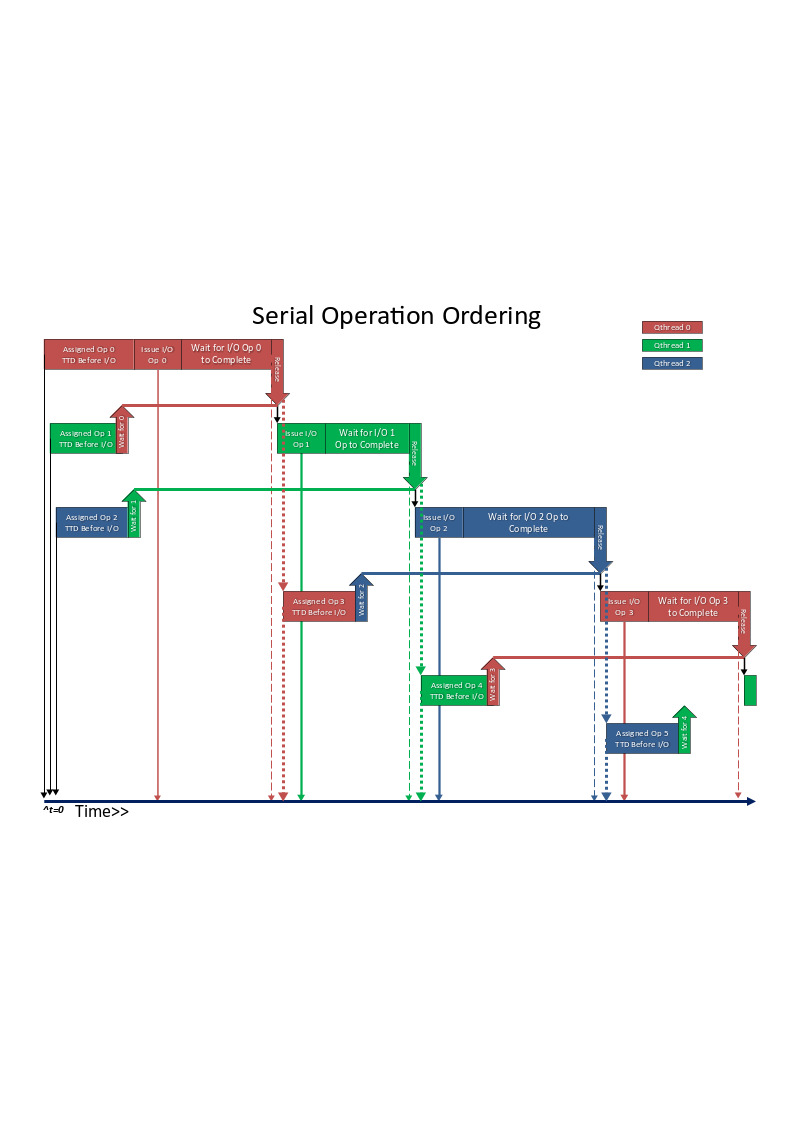
\includegraphics[width=7in,height=5.26736in,alt={Slide1.JPG}]{./images/media/image2.jpg}

\subsubsection{Loose Ordering}\label{loose-ordering}

Loose Ordering is similar to Serial Ordering but is not as strict. In Loose Ordering the QThread responsible for I/O Operation N+1 is supposed to issue its I/O Operation \emph{\ul{after}} I/O Operation N has been \emph{\ul{issued}} but \emph{\ul{before}} I/O Operation N has \emph{\ul{completed}}. The idea is that the storage controller will receive several I/O Operation requests and that after each request finishes, there is another request ready to be executed. There is also the distinct possibility that the subsequent I/O requests have some inherent locality of reference and the storage controller can optimize access to the storage devices based on this locality information.

For example, for purely sequential read operations, if the storage controller sees a consistent, well-ordered set of locations to access it will be able to perform read-ahead operations thereby maximizing the read bandwidth of the underlying storage subsystem. Similarly, for write operations the storage controller could use its write cache more effectively by taking several write operations and coalescing them into a single large write to the storage subsystem.

In practice, Loose Ordering seems to perform better than Serial Ordering for purely sequential read operations because the storage controller always has an I/O Operation to work on.

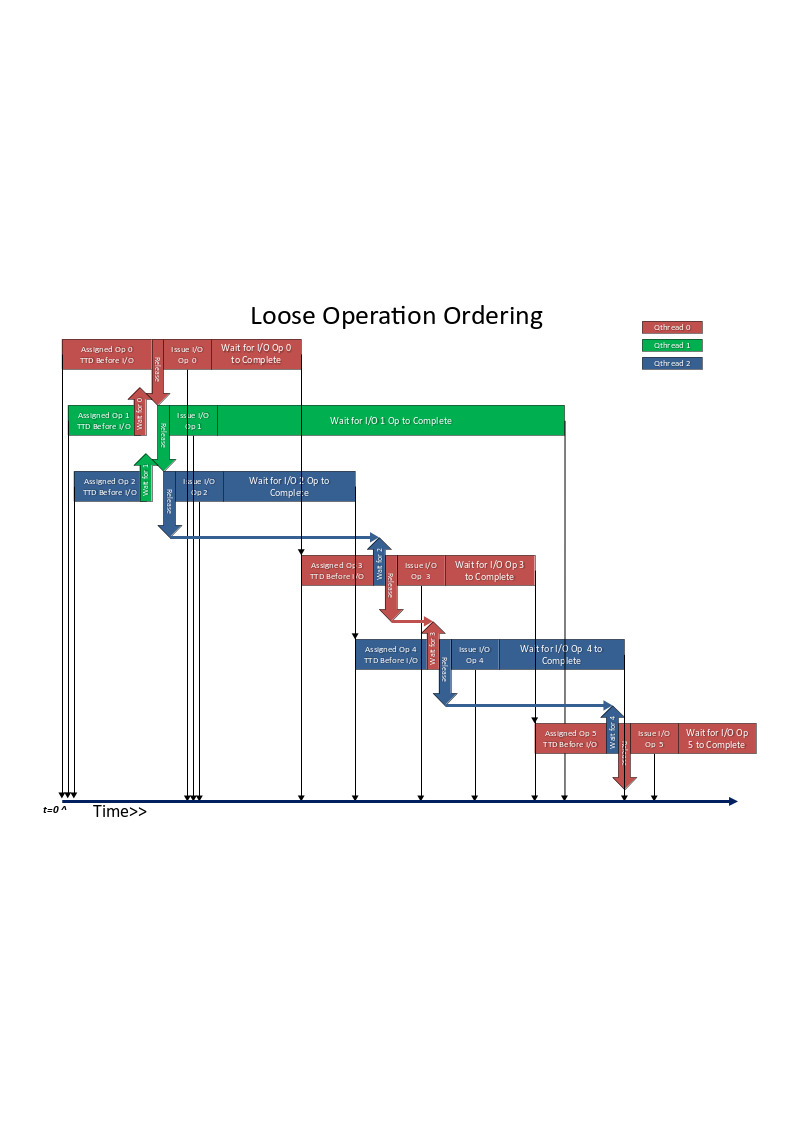
\includegraphics[width=7in,height=5.26736in,alt={Slide2.JPG}]{./images/media/image3.jpg}

\subsubsection{No Ordering}\label{no-ordering}

When No Ordering is used the QThreads will issue their respective I/O Operations without waiting for any prior I/O Operations to complete. The resulting order in which the storage controller sees I/O Operations should be reasonably sequential (in terms of order not necessarily in terms of access locations). However, the order in which the I/O Operations actually get issued depends largely on when the various QThreads are scheduled to run on the system. It has been observed that some QThreads can be ``starved'' for CPU cycles resulting in some I/O Operations experiencing long delays before they are issued and/or completed. This is more an artifact of the Operating System process scheduling algorithms than it is a property of XDD. If I/O Operation ordering is an issue, the Serial and Loose ordering schemes can be used.

